% 8-11(8쪽) — 정육면체 ABCD-EFGH 와 그 안의 삼각형 AFC. 스캔 화질이 낮아 TikZ 로 다시 그림(보이는 모서리 실선 · 숨은 모서리 점선 · 라벨은 원문의 꼭짓점 이름만).
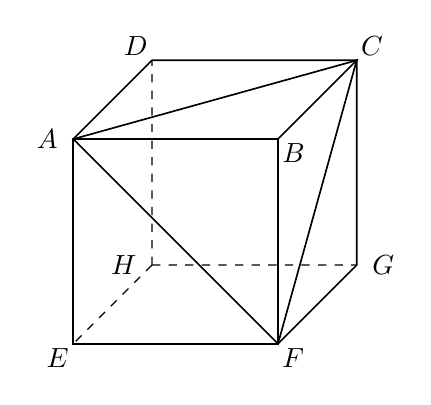
\begin{tikzpicture}[line width=0.6pt]
  \coordinate (A) at (0,2.6);
  \coordinate (B) at (2.6,2.6);
  \coordinate (F) at (2.6,0);
  \coordinate (E) at (0,0);
  \coordinate (D) at (1.0,3.6);
  \coordinate (C) at (3.6,3.6);
  \coordinate (G) at (3.6,1.0);
  \coordinate (H) at (1.0,1.0);
  \draw[dashed,line width=0.45pt] (H) -- (E) (H) -- (G) (H) -- (D);
  \draw (A) -- (B) -- (F) -- (E) -- cycle;
  \draw (A) -- (D) -- (C) -- (B);
  \draw (C) -- (G) -- (F);
  \draw (A) -- (C) -- (F) -- cycle;
  \node[above left=-2pt] at (D) {$\pt{D}$};
  \node[above right=-2pt] at (C) {$\pt{C}$};
  \node[left=2pt] at (A) {$\pt{A}$};
  \node[below right=-2pt] at (B) {$\pt{B}$};
  \node[left=2pt] at (H) {$\pt{H}$};
  \node[right=2pt] at (G) {$\pt{G}$};
  \node[below left=-2pt] at (E) {$\pt{E}$};
  \node[below right=-2pt] at (F) {$\pt{F}$};
\end{tikzpicture}
